\todo{Einstein puzzle as a running example? [T] if we call it holy zebra, makes sense to use Zebra as running example}

The \textbf{input} to \ourtool is a set of natural language sentences (from hereon referred to as ``clues''), and the names of the \textit{entities} that make up the puzzle, e.g. Englishman, red house, Zebra, etc.

In typical logic grid puzzles, this domain information is present in the grid that is supplied with the puzzle. For some puzzles, domain information is not required; a prototypical example is Einstein's Zebra puzzle, which ends with the question ``Who owns the zebra?'', while the clues do not name the Zebra entity, and the puzzle can be solved without knowledge of the fact that there is a zebra in the first place. 

%Figure \ref{fig:overview} contains an overview of the different components of the system.
%
%\begin{figure*}
%\centering
%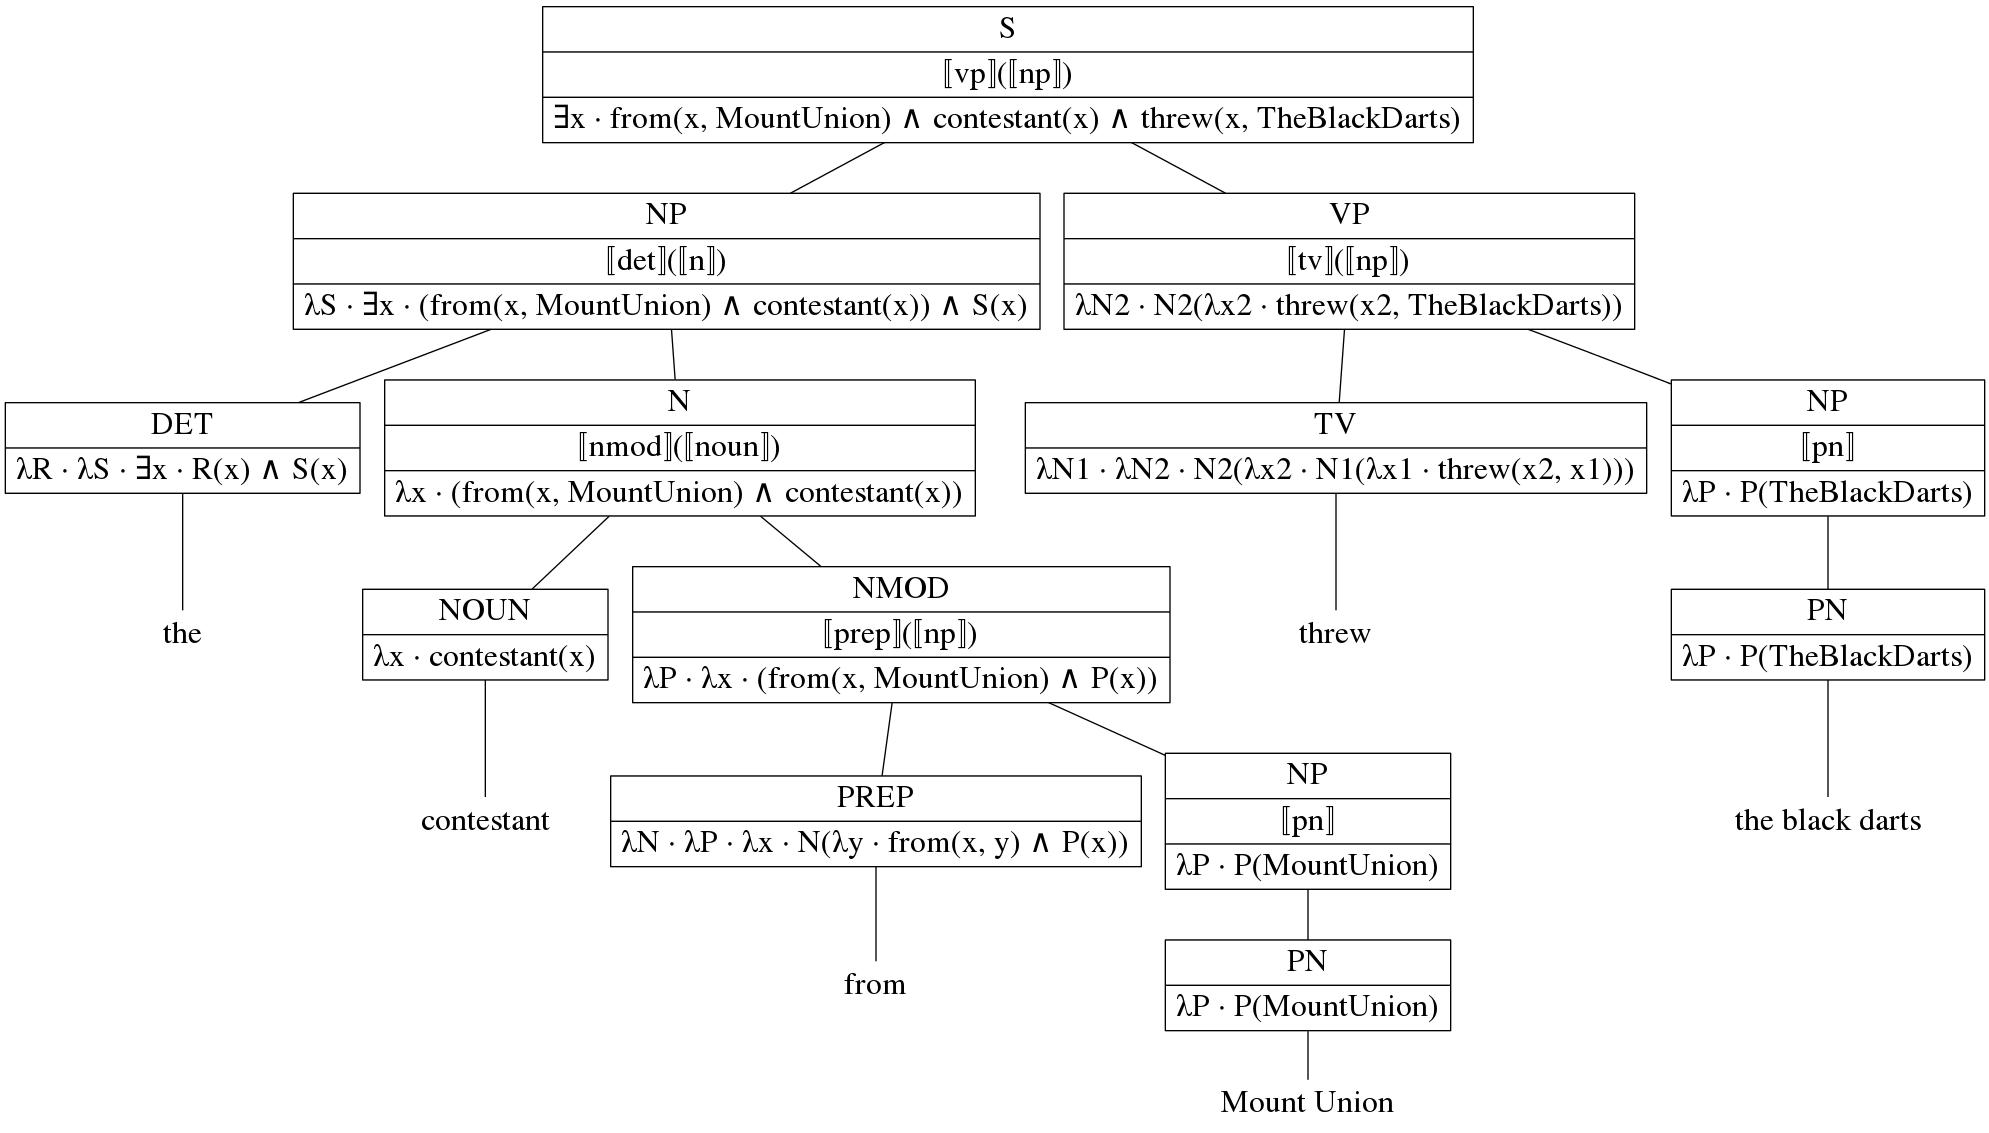
\includegraphics[width=\textwidth]{../../poster/graphviz/tree.jpg}
% Can someone replace this by a picture/schematic overview of the pipeline
% \caption{An overview of the pipeline of \ourtool.}
% \label{fig:overview}
%\end{figure*}

Our framework consists of the following steps, starting from the input:
\begin{enumerate}
\item Part-Of-Speech tagging
\item Chunking and lexicon building
\item From chunked sentences to logic
\item From logic to an IDP specification
\item Explanation-generating search in IDP
\item Visualisation of the explanation steps
\end{enumerate}

We now discuss each of these steps in turn.

\subsection{1. Part-Of-Speech tagging}
The standard procedure in Natural Language Processing is to start with tagging each word with its estimated Part-Of-Speech tag (POS tag). Standard tagsets exists, as do POS taggers.

We use the standard English Penn Treebank II POS tagset. As POS tagger we use NLTK's built-in Perceptron tagger~\footnote{http://www.nltk.org}. It uses a statistical inference mechanism, trained on a standard training set from the Wall Street Journal. As any POS-tagger can make mistakes, we make sure that all of the puzzle's entities are either tagged as \textit{noun} or \textit{adjective} depending on its use.

\subsection{2. Chunking and lexicon building}
To use the Blackburn \& Bos framework, a problem-specific \textit{lexicon} has to be provided, which assigns a role to different sets of words, and a problem-agnostic \textit{grammar} that reasons over these roles.

In prior work \todo{THESIS}, we identified a small set of primitives that covered the word usage in typical clues. The three central ones are: \textit{proper nouns}, namely the individual \textit{entities} that are central to the puzzle, \textit{other nouns} that refer to certain entities and \textit{transitive verbs} that refer to one or more entities.

Other primitives are \todo{For jens}. The \textit{transitive verb} category further contains \todo{For jens, tvPrep and tvGap}.

The goal of this second step is hence to group POS-tagged words into \textit{chunks} that are tagged with one of the above lexicon primitives. This process is known in the NLP community as \textit{chunking}. We use NLTK and a custom set of regular expressions for chunking the proper nouns and the different types of transitive verbs. \todo{PRIVATE NOTE: I did not actually implement this (yet?), but found out that this would be the right thing to do ; )}

The result is a lexicon, which is needed as input to the subsequent step in our framework. However, the POS tagging may be inaccurate and the chunking may also miss certain cases. Furthermore, logic puzzle authors are keen to use word play or seemingly ambiguous sentences to make the puzzle more interesting, and that require general world knowledge. For example, using 'in the morning' to refer to a timeslot at 11:00 when all other timeslots are after 13:00.

The automatically generated lexicon is hence tested as described in the next step, and if some clues can not be transformed into logic the user is asked to update the lexicon or rewrite a clue. For example, to replace 'in the morning' by 'at 11:00' in the earlier example.

\subsection{3. From chunked sentences to logic}

\todo{How does this relate to the next section? I might have screwed up the structure...}

3. (Adapted) Blackburn \& Bos
Input: [2. POS-rewriter]: the prolog fact with the rewritten sentences and the problem-specific lexicon
Static input (same for all the problems): the grammar that was derived during my thesis, the semantincs of a word-type (e.g. a verb has meaning X), the semantics of a grammar rule (how to combine the meaning of the words in case those words appear as in the grammar rule). Some of these semantics were provided by Blackburn \& Bos, some were added because they were logic puzzle specific. 
E.g. a sentence of the form "Of X and Y, one A and the other B" is defined in \url{https://github.com/bartbog/holygrail/blob/master/bos/myGrammarSemantics.pl#L33} and \url{https://github.com/bartbog/holygrail/blob/master/bos/myGrammar.pl#L91-L100} and is logic puzzle specific
Output: 
 - The First Order Logic representation of all the sentences
 - (Because it's adapted to have types): The types of all the words in the sentences

Blackburn \& Bos is a general framework with 4 inputs: lexicon, grammar, semantics for the lexicon (per word SORT, not per word!), semantics for the grammar. It works by combining the semantics of the words in the way that the semantics of the grammar specifies. It uses Discourse Representation Theory (DRT) for this because this captures quantors way better + it would work across sentences (not used in logic puzzles but this could capture the "He" in "Bart went jogging. He is tired" as "Bart"). The framework also provides a way to translate the DRT to FOL.

Because I adapted the framework, we also get a type for every word. E.g. for "Bart works in Brussels", it knows the subject of "works in" needs to be of the same type as "Bart" and the object of the same type as "Brussels". 

\subsection{4. From logic to an IDP specification}

\todo{How does this relate to the next section? I might have screwed up the structure...}


4. Transformer to IDP:
Input: Ouputs of [3. Blackburn \& Bos], MANUAL: the range of values for the numeric types.
Output: IDP translation of all the knowledge about the puzzle including:
- Typed FOL of all the sentences in the puzzle
- relations between the different predicate in the puzzle
- Typed FOL vocabulary
- (Some problem-specific lua code, but this is just glue)

A lot of this step is just glue to translate the FOL to IDP syntax. This step also does the following however:
- It unifies the different types (across sentences). E.g. "Bart works in Brussels" and "Jens works in Leuven", it will know that Jens and Bart need to be of the same type as the subjects of "works in" need to be off the same type (similar to all other verbs). 
- It detects synonyms (based on types) and add axioms to guarantee these are respected
- It adds some rules for transitive and reflexive relations (problem-specific but based on types!)
- It adds Logigram bijection axioms (not based on types)

This step still requires the range of values for the numeric types, all other questions can be eliminated in case the problem-specific lexicon mentions which ppn's are of the same type.


\subsection{5. Explanation-generating search in IDP}

\todo{How does this relate to the next-next section? I might have screwed up the structure...}


5. IDP Lua Code
Input: IDP Theory with the axioms + IDP Theory per sentence + Vocabulary
Output: Step-wise solution of the problem (including dependencies and sentence used to derive)

It tries to see what must hold given a theory and the axioms and a minimal set of things already known to be true/false. I hope Bart can give more info

6. Glue Code
(Not really important)
This just transforms the json from Bart a bit and saves it somewhere: \url{https://github.com/bartbog/holygrail/blob/master/bos/output/p2_types.output.json}
There is also a json from step 4 that lists all instances of all the types (grouped by type): \url{https://github.com/bartbog/holygrail/blob/master/bos/output/p2_types.voc.json}
-> It used the types for the latter but this could probably also be generated based on the input json

\subsection{6. Visualisation of the explanation steps}

\todo{How does this relate to the next-next section? I might have screwed up the structure...}

7. Visualization
Input: The 2 json's from above
Output: A step-wise visualization
% \end{verbatim}
